%% Make sure this figure winds up on page 2, even if you have to move
%% it to a different file.
\begin{figure*}[t!]
\centering
\subcaptionbox{Data flow. The user's browser uses Tor
  as a SOCKS proxy; Tor uses StegoTorus as \emph{its}
  SOCKS proxy. StegoTorus disguises the Tor link as innocuous
  cover-protocol traffic, perhaps split over many TCP connections,
  that pass through the perimeter filters and reach the StegoTorus
  server.  The server decodes the steganography and passes Tor
  traffic to the relay network.\label{f:dataflow}}%
[0.45\linewidth]{\centering%% Creator: Inkscape inkscape 0.48.3.1, www.inkscape.org
%% PDF/EPS/PS + LaTeX output extension by Johan Engelen, 2010
\begingroup%
  \setlength{\unitlength}{209.51999512bp}%
  \fontsize{8pt}{8pt}\selectfont
  \begin{picture}(1,0.86254295)%
    \put(0,0){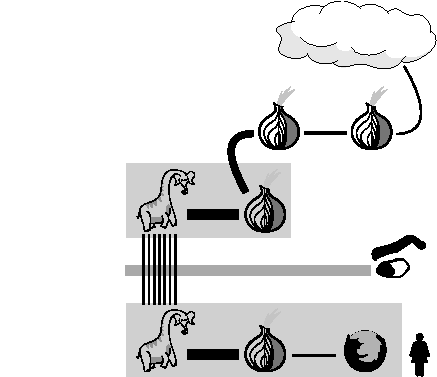
\includegraphics[width=\unitlength]{figures/dataflow}}%
    \put(0.14567428,0.09479557){\makebox(0,0)[b]{\smash{StegoTorus}}}%
    \put(0.14416226,0.23252598){\makebox(0,0)[b]{\smash{Censor}}}%
    \put(0.14567428,0.4152418){\makebox(0,0)[b]{\smash{StegoTorus}}}%
    \put(0.14571378,0.60323195){\makebox(0,0)[b]{\smash{Existing Tor}}}%
    \put(0.14591484,0.77214203){\makebox(0,0)[b]{\smash{Censored sites}}}%
    \put(0.14557659,0.56016918){\makebox(0,0)[b]{\smash{network}}}%
    \put(0.14569057,0.37224615){\makebox(0,0)[b]{\smash{server}}}%
    \put(0.14557918,0.05190503){\makebox(0,0)[b]{\smash{client}}}%
  \end{picture}%
\endgroup%
}%
\hspace{0.5cm}%
\subcaptionbox{Internal architecture.  The \emph{chopper} distributes
  re-encrypted Tor traffic to \emph{steganography modules}, which
  conceal it within cover-protocol messages.  Steganography modules
  can also generate decoy traffic directed at uninvolved hosts.
  Counterpart modules in the recipient decode the messages and
  reassemble the Tor link.  Both sides have access to independent
  \emph{covertext databases}.  Overall control rests with a
  configurable \emph{policy engine}.\label{f:arch}}%
[0.475\linewidth]{\centering%% Creator: Inkscape inkscape 0.48.3.1, www.inkscape.org
%% PDF/EPS/PS + LaTeX output extension by Johan Engelen, 2010
%% Accompanies image file 'arch.pdf' (pdf, eps, ps)
\begingroup%
  \setlength{\unitlength}{209.6bp}%
  \fontsize{7pt}{7pt}\selectfont
  \begin{picture}(1,0.8325522)%
    \put(0,0){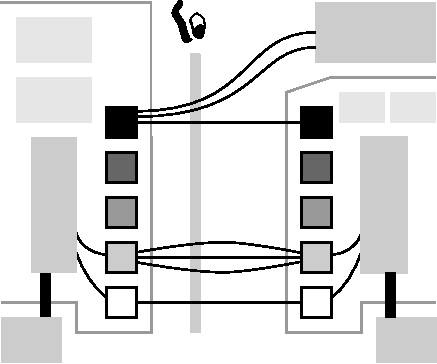
\includegraphics[width=\unitlength]{figures/arch}}%
    \put(0.475,0.7940151){\makebox(0,0)[lb]{\smash{Censor}}}%
    \put(0.1311603,0.36418277){\rotatebox{90}{\makebox(0,0)[b]{\smash{Chopper}}}}%
    \put(0.88688549,0.36418277){\rotatebox{90}{\makebox(0,0)[b]{\smash{Chopper}}}}%
    \put(0.82835114,0.58079374){\makebox(0,0)[b]{\smash{ct db}}}%
    \put(0.94671753,0.58079374){\makebox(0,0)[b]{\smash{pol en}}}%
    \put(0.28572519,0.70005326){\rotatebox{90}{\makebox(0,0)[b]{\smash{$\left.\rule{0pt}{11pt}\right\}\genfrac{}{}{0pt}{1}{\text{\fontsize{6pt}{6pt}\selectfont  Steganography}}{\text{\fontsize{6pt}{6pt}\selectfont modules}}$}}}}%
    \put(0.12359303,0.74901908){\makebox(0,0)[b]{\smash{Covertext}}}%
    \put(0.12409708,0.7156218){\makebox(0,0)[b]{\smash{Database}}}%
    \put(0.1241832,0.6146822){\makebox(0,0)[b]{\smash{Policy}}}%
    \put(0.12415816,0.58128695){\makebox(0,0)[b]{\smash{Engine}}}%
    \put(0.07224403,0.06220869){\makebox(0,0)[b]{\smash{Tor}}}%
    \put(0.07211212,0.02881384){\makebox(0,0)[b]{\smash{client}}}%
    \put(0.93102264,0.06227036){\makebox(0,0)[b]{\smash{Tor}}}%
    \put(0.93050355,0.02887435){\makebox(0,0)[b]{\smash{server}}}%
    \put(0.74234615,0.0338252){\makebox(0,0)[b]{\smash{StegoTorus}}}%
    \put(0.74157229,0.0004275){\makebox(0,0)[b]{\smash{server}}}%
    \put(0.26143011,0.03382518){\makebox(0,0)[b]{\smash{StegoTorus}}}%
    \put(0.2610434,0.0004273){\makebox(0,0)[b]{\smash{client}}}%
    \put(0.86109423,0.76926279){\makebox(0,0)[b]{\smash{Uncensored sites}}}%
    \put(0.86070205,0.73586663){\makebox(0,0)[b]{\smash{(decoy traffic)}}}%
  \end{picture}%
\endgroup%
}%
\caption{High-level overview of StegoTorus.}
\end{figure*}

\section{Architecture}\label{s:arch}

StegoTorus acts as a “pluggable transport”~\cite{s-tor-plugtrans} for
Tor, replacing its usual direct connection to a relay server.
Pluggable transport is an extension of SOCKS~\cite{s-socks}, so
StegoTorus could also camouflage traffic produced by other
applications that can use a SOCKS proxy. Figure~\ref{f:dataflow} shows
how the Tor$+$StegoTorus system transports data between the user's
browser and censored websites; Figure~\ref{f:arch} shows the internal
structure of the StegoTorus client and server.  StegoTorus applies two
additional layers of obfuscation to Tor traffic:

\textbf{Chopping} converts the ordered sequence of fixed-length “cells”
that Tor produces, into variable-length “blocks” that do not have to
be delivered in order. Each block is re-encrypted using a novel
cryptosystem geared for the needs of steganography: every byte of its
output is computationally indistinguishable from randomness.

Chopping can be used by itself for minimum overhead; since its
output has no predictable content and randomized packet sizes, this
is enough to defeat all known pattern filters and the attacks
described in Section~\ref{s:attacks}.  However, a pattern filter
that \emph{only} passes protocols with known, recognizable headers
would block it.

Chopping produces “blocks” that do not have to be delivered in order.
However, they must be delivered reliably.  At present, all our cover
protocols run over TCP.  StegoTorus cannot run directly over UDP, as
Dust does~\cite{c-dust}, but it could run over DCCP, or a UDP-based
cover protocol that provides reliable delivery.

\textbf{Steganography} disguises each block as a message in an innocuous
\emph{cover protocol}, such as an unencrypted HTTP request or
response.  Since blocks can be delivered out of order, StegoTorus
can distribute a Tor link over many cover connections, improving
both efficiency and difficulty of detection.  A StegoTorus server
can listen on many IP addresses, so that its clients appear to be
talking to many unrelated servers.  StegoTorus clients can generate
decoy traffic to uninvolved hosts, making detection even more
difficult.

\subsection{Design Goals}\label{s:threat}

\noindent
StegoTorus preserves Tor's basic design goals:

\smallskip
\begin{compactdesc}
\item[Unlinkability:] The censor should not be able to determine which
  Internet users communicate with which remote hosts via Tor.

\item[Performance:] Unlinkable access to the Internet should not be so
  much slower than “unmasked” access that users will reject the
  trade-off.

\item[Robustness:] The system should preserve its other design goals in
  the face of active attacks.
\end{compactdesc}

\smallskip\noindent
StegoTorus also seeks to provide:

\smallskip
\begin{compactdesc}
\item[Undetectability:] The censor should not be able to determine
  which Internet users are using StegoTorus.

\item[Unblockability:] The censor should not be able to block
  StegoTorus without also blocking a great deal of unrelated
  traffic.
\end{compactdesc}

\smallskip\noindent
The terms “unlinkability” and “undetectability” are defined precisely
by Pfitzmann and Hansen~\cite{s-anon-terms}.

\subsection{Threat Model}

We model a censorious adversary more or less as
Infranet~\cite{c-infranet} and Telex~\cite{c-telex} do.  A censor has
a \emph{network perimeter}, which cuts the global connectivity graph
into two disconnected components.  One of these components is “inside”
(or “censored”) and the other “outside.”  The censor controls all the
network infrastructure inside the perimeter, but \emph{not} the
software on end users' computers. (Attempts to mandate censorware on
end users' computers, such as China's 2009 “Green Dam” initiative,
have so far been unsuccessful~\cite{n-greendam}.)

The censor wishes to prevent the censored nodes from retrieving
material that meets some definition of undesirability; we assume that
no such material is \emph{hosted} inside the perimeter.

\subsubsection{Perimeter Filtering}

The censor programs the routers for all perimeter-crossing links to
observe all cleartext traffic that they forward.  This includes any
cleartext portion of a mostly-encrypted protocol, such as IP and TCP
headers and TLS record framing.  Using three general techniques, the
routers detect undesirable material and prevent it from crossing the
perimeter.

\begin{asparadesc}
\item[Address filters] prevent all communication with the IP addresses
  of servers that are thought to host undesirable material.  China
  maintains a blacklist of Tor entry nodes as part of its “Great
  Firewall.”

\item[Pattern filters] look for deterministic patterns in cleartext
  that may indicate undesirable material.  As mentioned in
  Section~\ref{s:intro}, Iran was able to block all use of Tor for a
  few weeks with a pattern filter looking for a particular
  Diffie-Hellman public modulus in TLS handshakes.

\item[Statistical filters] look for stochastic patterns, and can take
  low-level packet characteristics (size, arrival time, etc.)\ into
  account as well as cleartext headers and payloads.  While
  statistical filters for Tor are easy to construct (we describe one
  in Section~\ref{s:detect-tor}), we are not aware of any use of them
  in the field, to date.

\end{asparadesc}

\subsubsection{Limits on the Censor}\label{s:limits-censor}

Perimeter filtering must operate in real time on a tremendous traffic
volume.  To give some idea of the necessary scale, the CAIDA project's
“Anonymized Internet Traces 2011” data set~\cite{d-caida} consists of
the first \SI{64}{bytes} of every packet that traversed a backbone
router in Chicago for one hour on a Wednesday afternoon; there are
\SI{1.96}{billion\ packets} in the set, for a total of
\SI{116}{gigabytes} of data.  This corresponds to an average traffic
rate of \SI{540000}{packets} per second; a filtering router that needs
an extra two microseconds to process each packet will \emph{halve}
overall throughput.

The precise capabilities of commercial “deep packet inspection”
hardware are not widely advertised.  We assume, in general, that a
nation-state adversary has access to equipment that can perform a
two-stage analysis.  The first stage sees every packet, runs with a
hard realtime deadline, and must judge the vast majority of packets to
be uninteresting.  The second stage can only examine a tiny fraction
of the TCP flows crossing the router, and may be limited to responding
after-the-fact.  This is consistent with the observed behavior of
China's active probes for Tor bridges~\cite{n-china-active}.

We assume all Tor relays are outside the perimeter, and the censor
does not operate malicious Tor relays, nor does it observe traffic
among outside nodes.  If any of these assumptions are false, the
censor may be able to break Tor's unlinkability
guarantee~\cite{a-serve-surf,a-tor}.  StegoTorus obfuscates the
traffic between the Tor client and the first Tor relay. Since
the client is inside the perimeter, and the relay outside, StegoTorus
controls what the perimeter routers observe.

We also assume that the censor does not “turn off the Internet” (that
is, disconnect from the global network).  This \emph{was} done by
several countries during the Arab Spring, but only for a short time,
in response to imminent existential threat, and with negative
consequences for those who tried it.  We expect that other governments
will not repeat this mistake.  Similarly, we assume that address
filters prevent communication with only a relatively small number of
IP addresses.  Unlike systems such as Telex and
Cirripede~\cite{c-cirripede}, however, StegoTorus can potentially work
even if the only protocol allowed to cross the perimeter is
unencrypted HTTP.

It is difficult for two parties to communicate securely if they have
never communicated securely in the past.  Tor users must first obtain
the Tor client and learn the address of at least one relay, via some
extra-Tor method.  Similarly, StegoTorus users must obtain the
StegoTorus client (as well as the Tor client) and learn the address
and public key of at least one StegoTorus server.  We assume that
all necessary software and an initial server contact can be smuggled
over the perimeter, via “sneakernet” if necessary.

Since we anticipate that StegoTorus servers will be aggressively
blocked with address filters, we are developing a “rendezvous”
mechanism for distributing server address updates to StegoTorus
users~\cite{c-rendezvous}.  In this paper we assume that the user
knows contact information for server(s) that have not yet been
blocked.
